\documentclass[tikz,border=1.25mm]{standalone}
\usetikzlibrary{matrix, positioning, shapes, fit, shapes.geometric, backgrounds, arrows.meta}

\definecolor{cadmiumred}{rgb}{0.89, 0.0, 0.13}
\definecolor{kellygreen}{rgb}{0.3, 0.73, 0.09}
\definecolor{gray}{rgb}{0.54, 0.54, 0.54}
\definecolor{slate}{rgb}{0.094,0.094,0.112}

\begin{document}

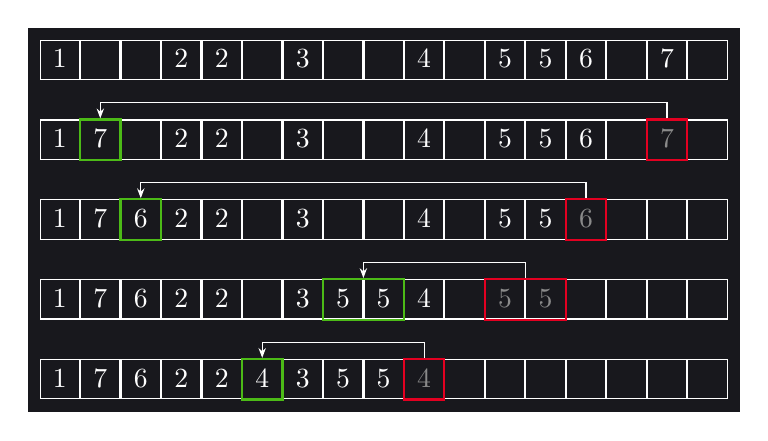
\begin{tikzpicture}[
  background rectangle/.style={fill=slate},
  show background rectangle,
  every node/.style={
    color=white,
    draw,
    inner sep=0mm,
    minimum height=5mm,
    minimum width=5mm,
    text height=2mm,
    text depth=0mm
  },
  removed/.style={
    draw=cadmiumred,
    thick
  },
  added/.style={
    draw=kellygreen,
    thick
  },
  move arrow/.style={
    -{Stealth[length=1.25mm]},
    draw=white
  }
]

\matrix[
	matrix of nodes,
	nodes in empty cells,
	column sep=0mm,
	row sep=5mm,
	draw=none
] (m) {
    1 &   &   & 2 & 2 &   & 3 &   &   & 4 &   & 5 & 5 & 6 &   & 7 &   \\
    1 & 7 &   & 2 & 2 &   & 3 &   &   & 4 &   & 5 & 5 & 6 &   & |[text=gray]| 7 &   \\
    1 & 7 & 6 & 2 & 2 &   & 3 &   &   & 4 &   & 5 & 5 & |[text=gray]| 6 &   &   &   \\
    1 & 7 & 6 & 2 & 2 &   & 3 & 5 & 5 & 4 &   & |[text=gray]| 5 & |[text=gray]| 5 &   &   &   &   \\
    1 & 7 & 6 & 2 & 2 & 4 & 3 & 5 & 5 & |[text=gray]| 4 &   &   &   &   &   &   &   \\
};

\node(rem1)[fit=(m-2-16), removed] {};
\node(rem2)[fit=(m-3-14), removed] {};
\node(rem3)[fit=(m-4-12)(m-4-13), removed] {};
\node(rem4)[fit=(m-5-10), removed] {};

\node(add1)[fit=(m-2-2), added] {};
\node(add2)[fit=(m-3-3), added] {};
\node(add3)[fit=(m-4-8)(m-4-9), added] {};
\node(add4)[fit=(m-5-6), added] {};

\coordinate[above=2mm of rem1] (rem1_up) {};
\coordinate[above=2mm of rem2] (rem2_up) {};
\coordinate[above=2mm of rem3] (rem3_up) {};
\coordinate[above=2mm of rem4] (rem4_up) {};

\coordinate[above=2mm of add1] (add1_up) {};
\coordinate[above=2mm of add2] (add2_up) {};
\coordinate[above=2mm of add3] (add3_up) {};
\coordinate[above=2mm of add4] (add4_up) {};

\draw[move arrow] (rem1) -- (rem1_up) -- (add1_up) -- (add1);
\draw[move arrow] (rem2) -- (rem2_up) -- (add2_up) -- (add2);
\draw[move arrow] (rem3) -- (rem3_up) -- (add3_up) -- (add3);
\draw[move arrow] (rem4) -- (rem4_up) -- (add4_up) -- (add4);

\end{tikzpicture}

\end{document}
